% !Mode:: "TeX:UTF-8"
% !Mode:: "TeX:UTF-8"
\newcommand{\thepage}{} % to silence a hyperref warning about pdfpagelabels
\RequirePackage[]{silence}
\WarningsOff[hyperref]
\PassOptionsToPackage{log-declarations=false}{xparse}
%\RequirePackage[l2tabu, orthodox]{nag}
\RequirePackage{luatex85} % to make \pdf...= commands work with LuaTeX
\documentclass[aspectratio=169,t]{beamer}
\usepackage{ifthen}
\usepackage[T1]{fontenc}
\usepackage{iftex}
\ifLuaTeX
 \usepackage{fontspec}
 \setmainfont[Ligatures=TeX]{Source Sans Pro}
\else
 \usepackage[utf8]{inputenc}
\fi
\usepackage{german}
\usepackage{newunicodechar}
\newunicodechar{€}{\texteuro}
\newunicodechar{ß}{\ss}
\renewcommand{\SS}{\iffontchar\font"1E9E \symbol{"1E9E}\else SS\fi}
\usepackage{ellipsis}
\usepackage{microtype}
\usepackage{listings}
\usepackage{sourcecodepro}
\lstset{language=Python, basicstyle=\ttfamily}
\usepackage{amsfonts}
\usepackage{amssymb}
\usepackage{amsthm}
\usepackage{fancyhdr}
\usepackage{graphicx}

\newtheorem{proposition}[theorem]{Proposition}

\DeclareMathOperator*{\argmax}{argmax}
\DeclareMathOperator{\supp}{supp}
\newcommand{\E}{\ensuremath{\mathbb{E}}}
\newcommand{\V}{\ensuremath{\mathbb{V}}}

\setbeamercolor{emph}{fg=purple}
\renewcommand<>{\emph}[1]{%
  {\usebeamercolor[fg]{emph}\only#2{\itshape}#1}%
}



\hypersetup{draft=false,colorlinks=false,pdfpagemode=UseOutlines,plainpages=false,
            breaklinks=true,bookmarksnumbered=true,pdfborder=0 0 0,
            pdftitle={Data Science SoSe 2026 HHU},
            pdfauthor={Konrad Voelkel},
            pdfsubject={data science}}

%\documentclass[aspectratio=169,t]{beamer}
\usetheme{hhubeamer} % put the hhu-beamer-theme in /usr/share/texmf/tex/latex/beamer/themes/

% -------------------- Code listings config --------------------
% Define custom colors for syntax highlighting
\definecolor{codegreen}{rgb}{0,0.6,0}
\definecolor{codegray}{rgb}{0.5,0.5,0.5}
\definecolor{codepurple}{rgb}{0.58,0,0.82}
\definecolor{backcolour}{rgb}{0.96,0.96,0.94} % Very light gray/beige
% Configure the listings package
\lstset{
    language=Python,
    backgroundcolor=\color{backcolour},   
    commentstyle=\color{codegreen}\itshape,
    keywordstyle=\color{blue}\bfseries,
    numberstyle=\tiny\color{codegray},
    stringstyle=\color{codepurple},
    basicstyle=\ttfamily\footnotesize, % Use a monospaced font
    breakatwhitespace=false,         
    breaklines=true,      
             % Enable automatic line breaking
    captionpos=b,                      % Caption at the bottom
    keepspaces=true,                 
    numbers=left,                      % Line numbers on the left
    numbersep=10pt,                    % Distance of line numbers from the code
    showspaces=false,                
    showstringspaces=false,            % Don't show weird underscores in strings
    showtabs=false,                  
    tabsize=4,
    frame=single,                      % Add a subtle border around the code
    rulecolor=\color{black!20},        % Border color
  }

\event[]{}
\author[Sommersemester 2026]{Dr. Konrad Völkel, Sommersemester 2026}

%\title{Data Science, VL 1}
%\date{16.04.2026}


%%% Local Variables:
%%% mode: latex
%%% TeX-master: t
%%% End:


\title{Data Science, VL 19}
\subtitle{Regression}
\date{25.06.2026}

\begin{document}

\begin{frame}
  \titlepage
\end{frame}

\section{Regression}

\begin{frame}[separator]
  \frametitle{Regression und Klassifikation}
\end{frame}


\begin{frame}
\frametitle{Klassifikation}
Klassifikation ist ein Oberbegriff für Supervised Learning Methoden,
bei denen die Zielvariable / die \alert{Label} kategorial verteilt (nominal skaliert) sind.

\vspace{1cm}

\uncover<2->{
Ziel ist, aus einem Trainingsdatensatz (mit gegebenen Labels) den Zusammenhang zwischen allen anderen Variablen mit den Labels zu 'lernen', um so für neue Daten (ohne Labels) das Label vorherzusagen / zu schätzen.
}

\vspace{1cm}

\uncover<3->{
  Um zu evaluieren, wie gut das 'lernen' geklappt hat, behalte einen Teil der Daten mit Label (\alert{train-test-split}),
  vergleiche Vorhersage mit 'ground truth'.
  }
\end{frame}

\begin{frame}
\frametitle{Beispiel zur Klassifikation}
Anhand der Blütenblattlänge (petal length) wollen wir die Iris-Spezies\\
'Setosa' (0) und 'Versicolor' (1) unterscheiden.

\uncover<2->{
  Variable: eine reelle Zahl, die Blütenblattlänge (petal length).

  Ziel/Label: 0 oder 1 ($\to$ \alert{binäre Klassifikation})
}

\vspace{0.5cm}

\uncover<3->{
  Aus einer Stichprobe 'lernen' wir z.B. dass Setosa Blütenblätter von Länge $< 2$ hat,
  Versicolor hingegen meist Länge $> 3$.

\vspace{1cm}
  
  Möglicher Klassifikator: $\texttt{prediction} = {[\texttt{petal\_length} < 2.5]}$
}

\uncover<2>{

  
\vspace{-2.5cm}
  
  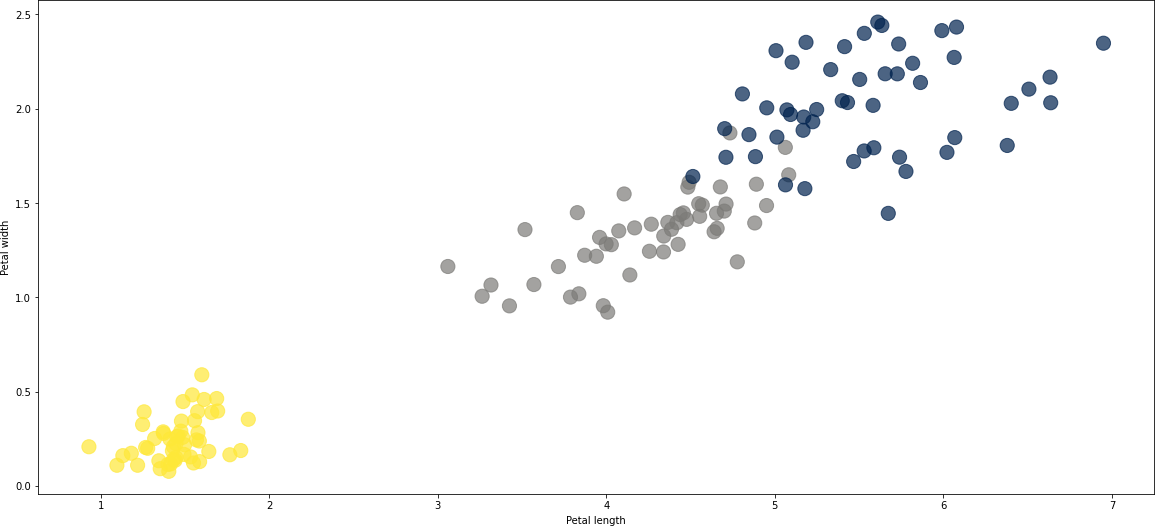
\includegraphics[height=3.5cm]{figures/iris-petal-plot.png}
  
  }
\end{frame}

\begin{frame}
\frametitle{Klassifikation vs. Clustering}
Während mit Klassifikation stets Supervised Learning, also bekannte Ziel-Variable mit vorliegenden Labels in Trainingsdaten gemeint ist,

\vspace{0.1cm}

ist Clustering eine Zuordnung zu Gruppen, die nicht in den Daten vorliegt.


\vspace{1cm}

\uncover<2->{
  Beim Clustering 'erfindet' man also Label bzw. die Labelvariable zählt nicht zu den beobachtbaren Variablen sondern ist \alert{latent} (= nicht beobachtbar).

  Clustering ist also Unsupervised Learning.
}

\vspace{0.5cm}

\uncover<3->{
  Supervised Learning ist viel einfacher zu evaluieren:

  Unterschied Vorhersage/Ground Truth.
  }
\end{frame}

\begin{frame}
\frametitle{Regression \uncover<4->{als Verallgemeinerung der Klassifikation}}
Regression ist ein Oberbegriff für Supervised Learning Methoden.

\uncover<4->{$\to$ Meist sind die Label kardinal skaliert, wenn man von Regression spricht.}

\vspace{0.6cm}

\uncover<2->{
Ziel ist, aus einem Trainingsdatensatz (mit gegebenen Labels) den Zusammenhang zwischen allen anderen Variablen mit den Labels zu 'lernen', um so für neue Daten (ohne Labels) das Label vorherzusagen / zu schätzen.
}

\vspace{1cm}

\uncover<3->{
  Um zu evaluieren, wie gut das 'lernen' geklappt hat, behalte einen Teil der Daten mit Label (\alert{train-test-split}),
  vergleiche Vorhersage mit 'ground truth'.
  }
\end{frame}

\begin{frame}
\frametitle{Beispiel zur Regression}
Anhand der Blütenblattlänge (petal length) wollen wir die Blütenblattbreite (petal width) vorhersagen.

\uncover<2->{
  Variable: eine reelle Zahl, die Blütenblattlänge (petal length).

  Ziel/Label: die Blütenblattbreite (petal width).
}

\vspace{0.5cm}

\uncover<3->{
  Aus einer Stichprobe 'lernen' wir z.B. dass die Breite ungefähr die halbe Länge minus $1$ ist.

\vspace{1cm}
  
  Möglicher Prädiktor: $\texttt{predicted\_petal\_width} = {\texttt{petal\_length}*0.5 - 1}$
}

\uncover<2>{

  
\vspace{-2.5cm}
  
  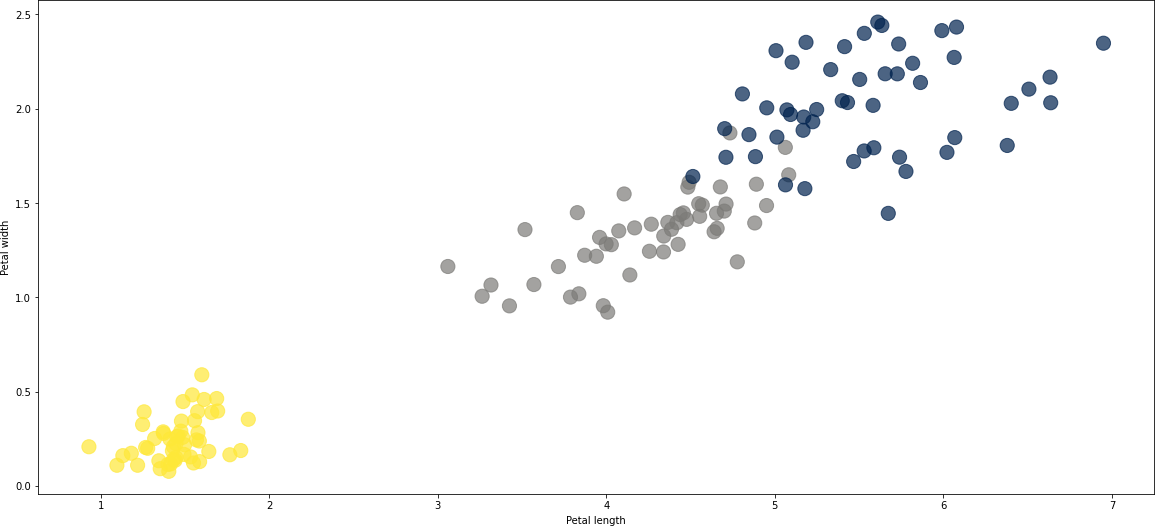
\includegraphics[height=3.5cm]{figures/iris-petal-plot.png}
  
  }
\end{frame}

\begin{frame}
\frametitle{Regressionsmodell, formal (Herleitung)}
Im Beispiel\\
$\texttt{predicted\_petal\_width} = {\texttt{petal\_length}*0.5 - 1}$\\
haben wir gesehen:

\vspace{0.7cm}

Vorhersage der Zielgröße = Funktion angewandt auf Einflussgröße

\vspace{0.5cm}

\uncover<2->{
 Parameter aus den Daten geschätzt, hier $0.5$ und $-1$
}

\vspace{0.7cm}

\uncover<3->{
  Dabei  haben wir nicht perfekt geschätzt, es gibt einen Fehler\\
  $\epsilon := \texttt{predicted\_petal\_width} - \texttt{petal\_width}$
}
\end{frame}


\begin{frame}
\frametitle{Regressionsmodell, formal}
  Ein \alert{Regressionsmodell} besteht aus:
  \begin{itemize}
  \item \alert{Regressoren} $X = (X_1,\dots,X_k)$, die 'unabhängige' Einflussgröße(n)
  \item \alert{Regressand} $Y$, die 'abhängige' Zielgröße
  \item \alert{Parametern} $\beta = (\beta_1,\dots,\beta_l)$
  \item \alert{Störgröße} $\epsilon$
  \item $Y = f(X; \beta) + \epsilon$ ist das eigentliche \alert{Modell}.
 \end{itemize}
  
\uncover<2->{
  Für eine konkrete Stichprobe haben wir Instanzen $x_1,\dots,x_N$ und Label $y_1,\dots,y_N$,
  wobei $x_{ij}$ der Wert von $X_j$ bei Instanz $i$ ist.
}

\uncover<3->{
  Die \alert{Vorhersage} $y_i^{pred} := f(x_i;\beta)$ hängt von den Parametern ab. \\
  Die Instanzen von $\epsilon$ sind die \alert{Residuen} $\epsilon_i = y_i - y_i^{pred}$.
  }
\end{frame}

\begin{frame}
\frametitle{Regression als Schätzer}
Gegeben eine Stichprobe von $X$, schätzen wir Parameter $\beta$ um eine möglichst gute Vorhersage für $Y$ zu erhalten.

\begin{itemize}
\item Die Regressionsmodelle unterscheiden sich in der Funktion $f$.
\item Eine \alert{Regressionsanalyse durchführen} heißt, ein Modell (d.h. eine Funktion $f$ und damit eine Anzahl Parameter) festzulegen und dann eine Schätzung für die Parameter aus der Stichprobe zu berechnen.
\item Meist soll $\beta$ so gewählt werden, dass $y_i^{pred}$ möglichst 'oft nah dran' ist an $y_i$.
\item <2->{
    Beispiel: wenn $\beta$ nur ein einzelner Parameter ist, und $f(x;\beta) = \beta$ die konstante Funktion,
    dann ist $Y = \beta + \epsilon$ das Modell (ein konstantes Modell).

    Mögliche Lösung: $\beta = \texttt{mean(X)}$.
  }
\end{itemize}
\end{frame}

\begin{frame}
  \frametitle{Achtung: Begriffe anderswo}
  \begin{itemize}[<+->]
  \item Eigentlich Klassifikation als Spezialfall der Regression\\
    Oftmals Regression = stetig vs. Klassifikation = diskret.
  \item Regression ganz allgemein, irgendein Modell mit Funktion $f$\\
    Oftmals Regression = lineare Regression, d.h. $f$ ist eine lineare Funktion
  \item Regression in vielen Dimensionen\\
    Oftmals Regression = in einer Dimension, Ergebnis ist eine \alert{Regressionsgerade}.
  \end{itemize}
\end{frame}


\begin{frame}
\frametitle{Unsupervised Regression?!}
So wie das Clustering die 'unsupervised Version' der Klassifikation ist,\\
was ist die 'unsupervised Version' der Regression?

\uncover<2->{
  $\to$ Das Berechnen einer neuen (z.B. stetigen) Variable aus den alten.

  Das ist eine Form von \alert{Feature Engineering}.
}

\vspace{1cm}

\uncover<3->{
  Das 'ultimative' unsupervised learning ist das Lernen der Verteilung,\\
  um so neue Samples generieren zu können.
}

\uncover<4->{
  Das ist mehr als nur Parameterschätzen:\\
  auch das Modell muss gewählt werden ($\to$ \alert{model selection}).
  }

\end{frame}



\begin{frame}[separator]
  \frametitle{Vielen Dank für Ihre Aufmerksamkeit!}
\end{frame}

\end{document}

%%% Local Variables:
%%% mode: latex
%%% TeX-master: t
%%% End:
